%this will contains the latex report
\documentclass{article}
\usepackage[utf8]{inputenc}
\usepackage{amsmath}
\usepackage{amsfonts}
\usepackage{xcolor}
\usepackage[allcolors=blue]{hyperref}
\usepackage{cleveref}
\usepackage{dirtytalk}

\newcommand\dhawat[1]{\textcolor{red}{DH: #1}}
\newcommand\mabaach[1]{\textcolor{magenta}{MA: #1}}
\newcommand\mboussaa[1]{\textcolor{blue}{MB: #1}}


\begin{document}
\section{Intoduction} % (fold)
\label{sec:Intoduction}
With any form of decision making, the quality of the decision is only as good as the data analysed, and so there is a need to ensure that the highest quality data is available for analysis. While having good levels of data quality improves analysis accuracy, having bad data quality can have a serious impact on the enterprise.
Poor data quality has a substantial impact, such as financial loss.  \href{https://www.ibm.com/blogs/journey-to-ai/}{IBM} estimate the loss of 3.1 trillion dollars annually  in USA due to poor data quality which is twice \href{https://data.worldbank.org/indicator/NY.GDP.MKTP.CD}{Canada’s GDP} in the very same year. Productivity loss, \href{https://www.forrester.com/report/Build-Trusted-Data-With-Data-Quality/RES83344}{Forrester} came up with a study that 40\% spend 1/3 of their time validating and fixing data quality issues. All of that lead to a low trust data.
Traditional data quality control methods are based on users’ experience or previously established business rules, and this
limits performance in addition to being a very time consuming process and low accuracy.

The main \mabaach{purpose} objective of this research \mabaach{is to examine the possible use of probability and machine learning techniques to .. ?} was to examine how can we use
probability models and machine learning to improve indicators
of data quality in a given dataset, with no \mabaach{without any prior knowledge of the domain ?} domain specific knowledge.
There was no particular regard to the domain of the dataset chosen, the main criteria for choice was the concept that bad data or outlier are rare data objects, \mabaach{\textit{i.e.}} i.e., those objects with rare combinations of feature values, compared to the majority of objects.
We built a package of Python algorithms to detect bad data present \mabaach{presence} in any type of table of data. \mabaach{Those} This algorithms are gathered in a Python class easy to use, and provided with detailed documentations, facilitating the comprehension and opening the door for further development of this class. The class contains test for many type of outlier (bad data) that could be found in a table of data such as: detection of repetition row, break of uniqueness rule, search for extreme values for columns with density distribution, non significant rows and columns, detection of spelling errors, and typographical error, outlier detection over rows, in each column and in each category of the columns with discreet distribution, detection of logical error between correlated columns.

This short survey is a report on the problem of data quality proposed by the company \href{ https://www.foyer.lu/en/homepage}{Foyer} during the challenges \href{https://challenge-maths.sciencesconf.org/}{\textit{mathematiques et entreprises}} organized by AMIES,  SFdS, SMF and SMAI.
In section \ref{sec:Data quality} we define \mabaach{what data quality is and different metrics used to asses it} the metrics describing the quality of data present in a table of data, and the difficulty arising while trying to find bad data, or to estimate the quality of the table in general. Then in section \ref{sec:Starategy used to detect bad data} we details our strategy used to deal with bad data. This section present theoretical mathematical concept behind the tests present in our Python package. In section \ref{sec:Algorithm}, we present some of the principal code used in our package described in section ref{sec:Starategy used to detect bad data}. In section \ref{sec:Experiments} we present the results of the test of our code on the table of data provides by the company \href{ https://www.foyer.lu/en/homepage}{Foyer} to test the efficiency of our methods. Finally, in section \ref{sec:Discussions}, we present the limitations of our algorithm and we propose solutions to overcome this limitations, and develope further the package.

% sectionIntoduction (end)

\section{Data quality} % (fold)
\label{sec:Data quality}
Let us first start with the heart of the problem, what can we consider as being good data? In an idyllic world, when we proceed to do data collection, there would be no duplication rows in the database, no missing values, no typos or illogical errors, in a sense, no human alteration of the picture that we are trying to capture from the real world. In classification issues more specifically, the data would be homogeneous and all classes would be equally represented. But of course that is not exactly what happens. \\
When speaking about data quality, several dimensions come to mind, as in \cite{amazon}, we could refer to the \textit{extension} of the data thus, focusing our attention on data values, or to the \textit{intension} of the data which represents the logical view of the database, the two dimensions are interconnected, the later is harder to measure, but highly influences the applicability of the extension's range of attributes.\\
In order to measure the quality of a database, one must consider several dimensions both regarding the extention and the intension side of the data, thus the quality of data could be related to different metrics such as the first and most obvious one that comes to mind would be \textit{redundancy} which refers to duplicated instances (\textit{i.e.} repeated rows or columns), then comes \textit{completeness} a.k.a. the comprehensiveness or wholeness of the data, it can be measured by the presence of null values (\textit{i.e.} or missing data), however it is important to consider it within the right context \say{indeed, in the schema of product category, the absence of a value for the attribute \texttt{shoe\_size} is not relevant for a product in the category \textit{notebooks}} \cite{amazon}, thus measuring the completeness is only relevant when the attribute is applicable. \\
\textit{Consistency} refers to whether the same data kept at different places do or do not match. \textit{Intra-relation constraints} define the range of admissible values within a column (\textit{i.e.}, a specific data type, an interval for numerical columns, or set of values for categorical ones.), \textit{Inter-relation constraints} represents the logical inter-connectivity and interrelationship of the columns, then comes \textit{Accuracy}, which refers to whether the data values stored for an object are the ``correct values''. To be correct, a data values must be the right value and must be represented in a consistent and unambiguous form. there are two characteristics of accuracy: form and content. Form eliminates ambiguities about the content (\textit{i.e.} \texttt{BIRTH\_DAY} would have different format depending on which representation we choose, USA or European), and content accuracy compares the value of a column with its real world representation (\textit{i.e.} both 07/09/1993 and 09/07/1993 are valid in the context of \texttt{BIRTH\_DAY}), we can also mention other dimensions of data quality like the \textit{amount of data (imbalanced class), heterogeneity, reliability} (for example the year of birth is smaller than the year of the death), \textit{relevance} and \textit{timeliness}. \\
When dealing with data quality, we first need to assess the type of the data, distinguishing between \textit{categorical} and \textit{continuous} is vital, indeed the data type would highly influence the kind of errors we would be looking for (for nominal data one can check for typo errors (accuracy content dimension), for ordinal data the Intra-relation constraints would be important to acknowledge, for the continuous data, one would be looking for outliers using the data distribution). It would also influence the algorithmic techniques and tests that we would choose to apply. \\
Regarding outlier detection, the problem we are faced with is that in order for statistical techniques to work, we need to first assume that
\textit{almost surely}
the data is clean, thus the outlier behavior would be different enough that it would appear as an observation that was generated by a different mechanism as Hawkins officially defined it \cite{Hawking}.
Thus, it is necessary to combine deterministic approaches along with statistical ones to detect outliers, therefor we first need to ``clean'' the data by performing a serie of deterministic tests, identifying data behavior that ``obviously'' .
deviates from the ``norm'' for example if 99.99\% of the values of \texttt{column\_a} are higher than the values of \texttt{column\_b} it would mean that the remaining 0.01\% might be errors, which lead us to the section where we present the different strategies that we adopted to assess data quality.
\section{Starategy used to detect bad data}
\label{sec:Starategy used to detect bad data}



\subsection{Duplication test diala} % (fold)
\label{sub:Duplication test}


\subsection{Typographic test} % (fold)
\label{sub:Typographic test}
<<<<<<< HEAD
<<<<<<< HEAD
Detecting typo errors in strings is a tricky matter that relies on many factors such as how do we define similarities between strings. 
\subsubsection{Affinity propagation algorithm}
The first method we explored is clustering the words using a similarity matrix, it is a direct approach of the problem, it consists on first computing a similarity matrix between all the strings of the database, and then clustering them using a clustering algorithm that would not require the number of clusters as a parameter. After experimenting with many distances, we opted for the method \texttt{ratio} of the class \texttt{SequenceMatcher} from the python module\texttt{difflib} which showed the best results, this method return a measure of the sequences similarity, where $T$ is the total number of elements in both sequences, and $M$ is the number of matches, the method returns $\cfrac{2*M}{T}$ the downside of the method would be that it is computationally expensive, although it is possible to use the function \texttt{real\_quick\_ratio\(\)} which returns an upper bound on \texttt{ratio()} 
but this will impact the effectiveness of the method. Once we computed the similarity matrix, we use a method \texttt{AffinityPropagation} of the class \texttt{cluster} of the library \texttt{sklearn} \cite{sklearn}, which is to cluster the data, which is unsupervised machine learning algorithm that does not require the user to specify the number of clusters, based on the concept of ``message passing'' between data points, they can be seeing as a network where all data send messages to all other points. The subject of these messages are the willingness of the points being exemplars. Exemplars are points that explain the other data points ‘best’ and are the most significant of their cluster \cite{richi}. After the clustering, we would get count the number of occurences in each element of the cluster and decide that all elements that appear below a fixed threshold to be misspelling errors. The problem with the technique relies on the fact that it is hard to pick the ``right'' distance between the strings, one possibility would be to run the algorithm in each cluster after computing the similarity matrix of the cluster doing a second pass of the algorithm, empirical tests shows that it seems to work better, but further investigation are necessary.
The second method we proposed is based on a Markov clustering algorithm.
\subsubsection{Markov clustering}
The first step is to transform the data into a suitable format by doing feature extraction using \texttt{CountVectorizer} method from  \linebreak \texttt{sklearn.feature\_extraction.text} class, \cite{vector} which convert a collection of text documents to a matrix of token counts (\textit{i.e.} a token is an object that holds the place of something else that is usually larger or more complex.), Then we proceed and initialize an object of the \texttt{MarkovClustering} class \cite{MarkovClustering} and use it to perform a type of graph clustering using \textbf{Markov Chain theory} by first creating a \textbf{probability matrix of transition} then simulating a random walk by alternating between two operations \textbf{inflation} that would change the probability of transition to advantage strong neighbors and disadvantage weak ones and \textbf{expansion} that would connect different regions of the graph, it would repeat this process until the state of equilibrium is reached and the algorithm converges \cite{explainMCL}, after that we get the clustered data and apply the same technique as before to detect the misspelled words.\\
The problem with this technique is that the accumulation of hidden layers makes it difficult to assess why it works extremely well in some cases and it does not in others.
\subsection{Extreme values :diala} % (fold)
=======

=======
Detecting typo errors in strings is a tricky matter that relies on many factors such as how do we define similarities between strings, or how to encode strings in numerical values in an isometric way, the first method we investigated is called Affinity propagation technique.
\subsubsection{Affinity propagation algorithm}
The first method we explored is clustering the words using a similarity matrix, it is a direct approach of the problem, it consists on first computing a similarity matrix between all the strings of the database, and then clustering them using a clustering algorithm that would not require the number of clusters as a parameter. After experimenting with many distances, we opted for the method \texttt{ratio()} of the class \texttt{SequenceMatcher} from the python module\texttt{difflib} which showed the best results, this method return a measure of the sequences similarity, where $T$ is the total number of elements in both sequences, and $M$ is the number of matches, the method returns $\frac{2*M}{T}$ the downside of the method would be that it is computationally expensive, although it is possible to use the function \texttt{real\_quick\_ratio()} which returns an upper bound on \texttt{ratio()}
but this will impact the effectiveness of the method. Once we computed the similarity matrix, we use a method \texttt{AffinityPropagation} of the class \texttt{cluster} of the library \texttt{sklearn} \cite{sklearn}, which is to cluster the data, which is unsupervised machine learning algorithm that does not require the user to specify the number of clusters, based on the concept of ``message passing'' between data points, they can be seeing as a network where all data send messages to all other points. The subject of these messages are the willingness of the points being exemplars. Exemplars are points that explain the other data points ‘best’ and are the most significant of their cluster \cite{richi}. After the clustering, we would get count the number of occurences in each element of the cluster and decide that all elements that appear below a fixed threshold to be misspelling errors. The problem with the technique relies on the fact that it is hard to pick the ``right'' distance between the strings, one possibility would be to run the algorithm in each cluster after computing the similarity matrix of the cluster doing a second pass of the algorithm, empirical tests shows that it seems to work better, but further investigation are necessary.
The second method we proposed is based on a Markov clustering algorithm.
\subsubsection{Markov clustering}
The first step is to transform the data into a suitable format by doing feature extraction using \texttt{CountVectorizer} method from the \texttt{sklearn} class which is \texttt{feature\_extraction.text} \cite{vector} which convert a collection of text documents to a matrix of token counts (\textit{i.e.} a token is an object that holds the place of something else that is usually larger or more complex.), Then we proceed and initialize an object of the \texttt{MarkovClustering} class \cite{MarkovClustering} and use it to perform a type of graph clustering using \textbf{Markov Chain theory} by first creating a \textbf{probability matrix of transition} then simulating a random walk by alternating between two operations \textbf{inflation} that would change the probability of transition to advantage strong neighbors and disadvantage weak ones and \textbf{expansion} that would connect different regions of the graph, it would repeat this process until the state of equilibrium is reached and the algorithm converges \cite{explainMCL}, after that we get the clustered data and apply the same technique as before to detect the misspelled words.\\
The problem with this technique is that the accumulation of hidden layers makes it difficult to assess why it works extremely well in some cases and it does not in others.
>>>>>>> 1ab9d33075503ba03f5154c28769c0f190de65bc
% subsectionTypographic test (end)

\subsection{Extreme values diala} % (fold)
\label{sub:Extreme values}
\begin{figure}[H]
    \centering
    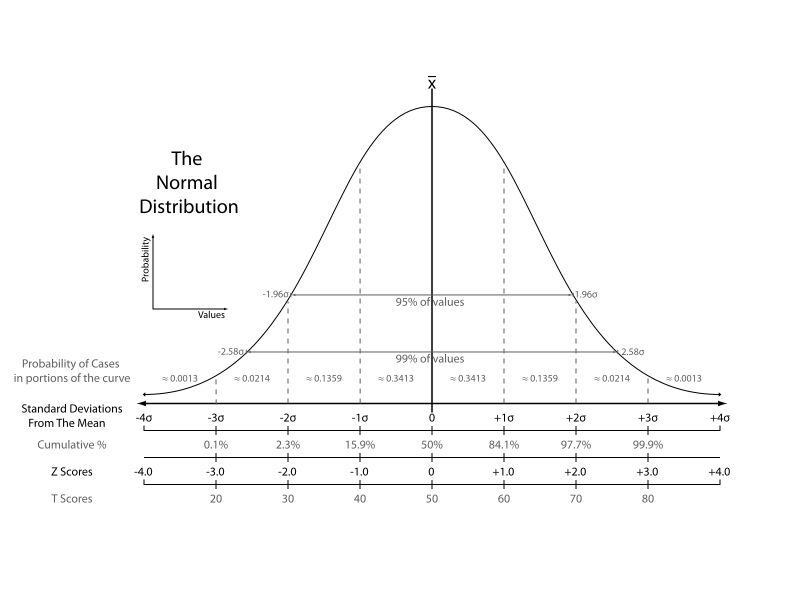
\includegraphics[width=0.8\linewidth]{picture/normal.png}
    \caption{Normal distribution.}
    \label{fig:normal}
\end{figure}
Probabilistic and statistical models can be used for outlier detection, including normal distribution and Zipf distribution. Moreover, these models work well in one-dimensional and
multidimensional data \cite{dai_yosh_pars}.
Statistical process control is a procedure of quality control, and it is based on statistical methods.
A normal distribution is a symmetric, continuous, bell-shaped distribution of a variable, displays a normal probability distribution as a model for a quality characteristics with the specification limits at three or six standard deviations $\sigma$ on either side of the mean $\mu$.
For example, within one standard deviation of the mean will cover 68\% of the data, while within 3 standard deviations from the mean will cover 99.73\% and within 6 standard deviation standard deviation of the mean will cover more then 99,99\% of the distribution
We use test of extreme values based on the above idea to find outliers present in a numerical column by finding its mean and standard deviation and rejecting values outside 6 standard deviation standard deviation of the mean.
We refer to this values as extreme values. Note that this test is applied to non constant numerical columns non unique and not discrete (i.e. columns without clustering aspect). This conditions prevent doing the test on distributions far from being Gaussian.

% subsection Extreme values (end)

\subsection{Completeness diala} % (fold)
\label{sub:Completeness}

% subsectionCompleteness (end)

<<<<<<< HEAD
\subsection{Total order relation: mariem} % (fold)
\label{sub:Total order relation}
The idea behind this algorithm is to find ordering errors between two numerical columns by detecting if there is an inherent order between them and flagging elements that does not respect it. For example all the values of the column \texttt{BIRTH\_YEAR} should be lower than there corresponding value in the column \texttt{DEATH\_YEAR}. We proceed to a tendency test between all numerical columns, let \texttt{column\_a} and \texttt{column\_b} be two numerical columns, we compute the ratio between the number of elements in \texttt{column\_a} that are lower to there corresponding in \texttt{column\_b} (row-wise comparison) and the length of the columns. We start by dropping the missing values first to avoid any problems. if the ratio is high that would mean that there is a hidden tendency between those two columns and that the values that does not respect that order might be outliers
=======
\subsection{Logical order relation: mariem} % (fold)
\label{sub:Logical order relation}
The idea behind this algorithm is to find ordering errors between two numerical columns by detecting if there is an inherent order between them and flagging the elements that does not respect it. For example all the values of the column \texttt{BIRTH\_YEAR} should be lower than there corresponding value in the column \texttt{DEATH\_YEAR} if not then it is an error. We proceed to a what we would call a tendency test between pairs of all numerical columns, let \texttt{column\_a} and \texttt{column\_b} be two numerical columns, we compute the ratio between the number of elements in \texttt{column\_a} that are lower to their corresponding value in \texttt{column\_b} (row-wise comparison) and the length of the columns. We start by dropping the missing values first to avoid any problems. if the ratio is high (let's say 99.99\% the threshold is a parameter that needs to be fixed to avoid too much false positives) that would mean that there is a hidden tendency between those two columns and that the values that does not respect that order might be outliers.
% subsection Logical order relation (end)
>>>>>>> 1ab9d33075503ba03f5154c28769c0f190de65bc

\subsection{Outlier detection with machine learning diala} % (fold)
\label{sub:Outlier detection with machine learning}
\begin{figure}[H]
    \centering
    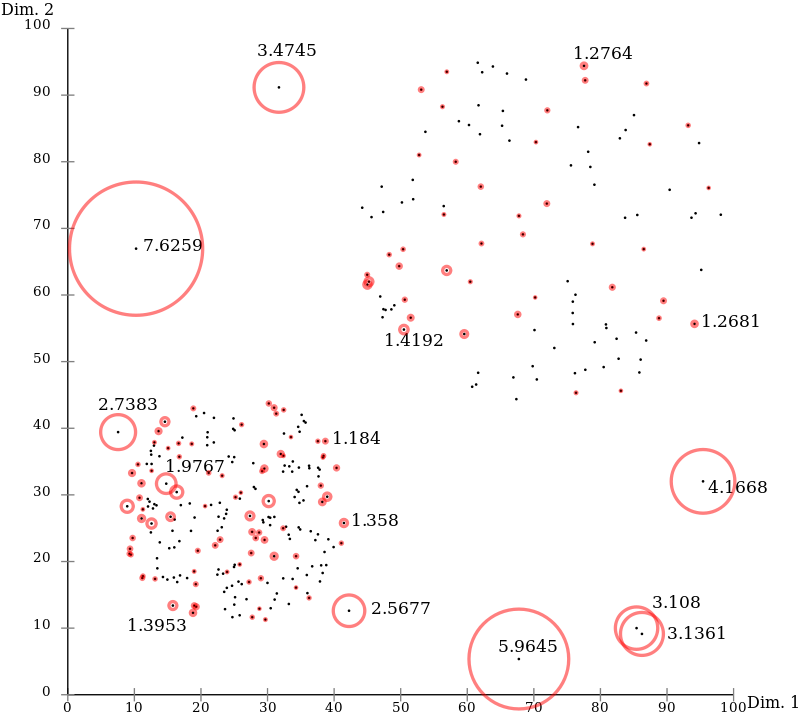
\includegraphics[width=0.6\linewidth]{picture/lof.png}
    \caption{Local Outlier Factor.}
    \label{fig:lof}
\end{figure}
The local outlier factor, or LOF for short, is a technique that attempts to harness the idea of nearest neighbors for outlier detection.
It is an unsupervised machine learning anomaly detection method.
The local outlier factor is based on a concept of a local density, where locality is given by k nearest neighbors, whose distance is used to estimate the density.
By comparing the local density of an object to the local densities of its neighbors, one can identify regions of similar density, and points that have a substantially lower density than their neighbors. These are considered to be outliers.
The local density is estimated by the typical distance at which a point can be ``reached" from its neighbors.
The definition of ``reachability distance" used in LOF is an additional measure to produce more stable results within clusters.
Due to the local approach, LOF is able to identify outliers in a data set that would not be outliers in another area of the data set.
For example, a point at a ``small" distance to a very dense cluster is an outlier, while a point within a sparse cluster might exhibit similar distances to its neighbors.
The LOF test is available in our Python package by the class method \texttt{check\_outlier}.
This test is applied on the numerical columns gathered.
Or the table contains \texttt{NaN} in the numerical columns and the LOF test does not apply to data containing missing values, we were facing the problem of dealing with the missing element before being able to to detect outliers by the LOF.
To overcome the problem of missing values data scientists use \textbf{imputation} methods.\\

\noindent
The imputation is process for fills missing data with synthetic values.
Imputation preserves all cases by replacing missing data with an estimated value based on other available information.
Once all missing values have been imputed, the data set can then be analysed using standard techniques for complete data.
There are different approach for imputing missing values \cite{corr_lede}:
\begin{enumerate}
    \item Deletion: removes all instances with missing values.
    \item Hot deck: missing data are filled with values from the same dataset.
    \item Imputation based on missing attributes: computes a new value from measures of central tendency as median, mode, mean,
          etc. The computed value is used for filling the missing data.
    \item Imputation based on non-missing attributes: a classification or regression model is built from available data to fill the missing values.
\end{enumerate}
Or for some table all rows contains missing values or most of them so the deletion option could not be used in the case were we are doing imputation over the hole table and not a specific columns.
From the last 3 methods we chose the imputation based on non-missing attributes using k-Nearest Neighbors provided by \href{https://scikit-learn.org/stable/modules/generated/sklearn.impute.KNNImputer.html}{sklearn}.
Missing values are imputed using the mean value from k-nearest neighbors found in the table. Two samples are close if the features that neither is missing are close.
% subsection  Outlier detection with machine learning (end)
\subsection{Frequency for logical errors diala} % (fold)
\label{sub:Frequency for logical errors}
As we already mentioned the step of detecting rows outlier of type logical error was done via the algorithm LOF preceded by an imputation method \ref{sub:Outlier detection with machine learning}.
Although finding the logical errors in a table (rows) is a difficult task in outlier detection, specifying there positions (rows, columns) is the most difficult task.
So we decide to flip the question maybe in that way the most difficult will be less difficult.
Based on the idea that outliers occur less then inliers, we construct an algorithm to detect logical error  between couples of correlated rows in this way we specify directly the positions (rows, columns) of a part of the logical error and we overcome the difficulty of this task.
We introduce a pattern-based methods, which search for outlying/normal patterns and employ pattern frequency as a direct outlierness measure to detect outliers.
For sufficiently 2 correlated columns, the idea is to find for each element of the first column the associated elements from the second columns and find the frequency of the couple and flag couples with sufficiently low frequency.
\begin{figure}[H]
    \centering
    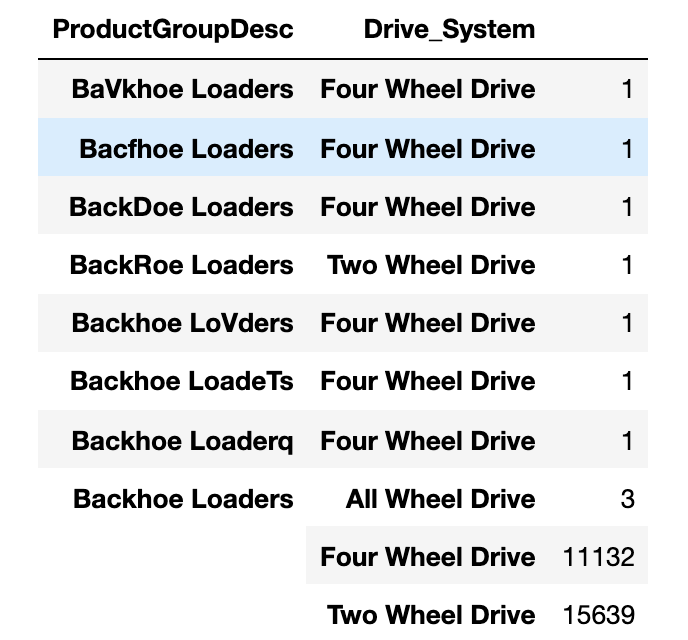
\includegraphics[width=0.6\linewidth]{picture/logic_err.png}
    \caption{Groups from 2 correlated columns.}
    \label{fig:logic_err}
\end{figure}
To simplify the idea we will consider an example from the table that we were provided. Figure \ref{fig:logic_err} represent the a sequences of couple of element from the columns \texttt{ProductGroupDesc} and \texttt{Drive\_system} and the frequency of occurences of each couple.
As we already mention the basic idea of outlier detection is that, in any table of data outlier occur less frequently then inlier.
By examining the frequencies of the the couple associated to \texttt{Backoe Loeders} we can deduce that \texttt{All Wheel Drive} occur clearly less then other frequencies and so it's an logical error. Moreover the high number of clusters in this column (11132, 15639) implies that all couples occurring 1 times are outliers, in this way we can also detect the spelling errors in the column \texttt{ProductGroupDesc} present in figure \ref{fig:logic_err} as the variant of \texttt{Backoe Loeders}
The same is applied for couple of categorical correlated
The test for detecting outlier of type logical error using the frequency is applied on couples of sufficiently correlated string columns, non unique, with categorical discrete aspect i.e. columns with clustering aspect.
As we already mentioned this algorithm we be held only on sufficiently correlated clustered columns, it is preceded by finding the matrix of correlations between sufficiently clustered  categorical columns.
% subsection Frequency for logical errors (end)

\subsection{Intra categorical extreme values mariem} % (fold)
\label{sub:Intra categorical extreme values}
We proceed as in \ref{sub:Frequency for logical errors} applying a pattern-based method between categorical columns and numerical ones, to look for extreme values within a specific class of a category (\textit{e.g.} the distribution of the price of a specific in class of the column \texttt{CAR}.). In order to do that we start by selecting categorical columns that contain very few classes (their ratio of uniqueness would be lower than a fixed threshold), and for a category column and a given numerical column, we partition the values of the numerical column using the classes of the categorical one we get $m$ subsets, $m$ being the number of classes in the categorical column: $\{c_1: n_{1, c_1}, n_{2, c_1}, \ldots, n_{i, c_1}\}, \ldots, \{c_m: n_{j+1, c_m}, \ldots,  n_{l, c_m}\}$ with $c_1, \ldots, c_m$ the classes of the categorical column and $(n_i)_{i \leq l}$ the values of the numerical one. Then we proceed to an extreme value test on each subset.
It is very important to distinguish between continuous numerical columns and the discrete ones because the testing procedure will not be the same, for the continuous numerical column we would use a \texttt{z-score} test and for the discrete ones we use the frequency of occurrences as in \ref{sub:Frequency for logical errors}.
% subsection Intra categorical extreme values (end)

% section  Starategy used to detect bad data (end)

\section{Algorithm medi} % (fold)
\label{sec:Algorithm}
Different error types and data types force us to use different methods and algorithm to judge data quality. In light of this we decided to split our algorithm into several standalone module capable of being called independently of one another.
If the user wishes to simply use all the algorithm and with standard parameters we provided two methods for doing so. The first method is used to get rid of easier to detect errors such as duplicates and typos before (if wished) passing it's results to the second method which will be a more in depth check.
Let us then follow our outlined methods and inspect the first method algorithms.


\subsection{First method}
\subsubsection{Duplicate errors algorithm}
\subsubsection{Typographical error algorithm}

\begin{algorithm}[H]
    \SetKwData{Left}{left}\SetKwData{This}{this}\SetKwData{Up}{up}
    \SetKwFunction{Union}{Union}\SetKwFunction{FindCompress}{FindCompress}
    \SetKwInOut{Input}{input}\SetKwInOut{Output}{output}
    \Input{A column of a DataFrame, a minimum frequency threshold, A specified method to deal with clustering}
    \Output{Index of the DataFrame containing typographical errors}
    \BlankLine

    list\_incorrect$\leftarrow$ [~]\;
    words $\leftarrow$ get unique element from input column\;
    \If{method is affinity propagation}
    {
        lev\_similarity $\leftarrow$ \lForEach{element $w1$ in word, element $w2$ in word}{SequenceMatcher(w1, w2)}
        affprop $\leftarrow$ instance AffinityPropagation\;
        affprop\_label $\leftarrow$ affprop.fit(lev\_similarity).labels \;
        \eIf{affprop\_label is empty}
        {
            return list\_incorrect\;
        }
        {\For{cluster in affprop\_label}
            {list\_incorrect $\leftarrow$ list\_incorrect + incorrect\_grammar(column, cluster, threshold)\;}
        }
        return list\_incorrect
    }
    \Else{
        X $\leftarrow$ instance Vectorizer and transform words into it\;
        dict\_cluster $\leftarrow$ get clusters from MarkovClustering(X)\;
        \If{dict\_cluster is empty}
        {return list\_incorrect}
    }
    \caption{Typographical checking\label{typo}}
\end{algorithm}



\subsubsection{Extreme value algorithm}

\begin{algorithm}[H]
    \SetKwInOut{Input}{input}\SetKwInOut{Output}{output}
    \Input{A column of a DataFrame, a minimum frequency threshold, The uniqueness ratio of the column, A standard deviation multiplie, 2 uniqueness thresholds}
    \Output{Index of the DataFrame containing extreme values}
    \BlankLine

    \uIf{uniqueness $\geq$ threshold\_1 or uniqueness $\leq$ threshold\_2}{return [~] \;}
    \Else{
        mean $\leftarrow$ mean(column)\;
        std $\leftarrow$ std(column)\;

        upper\_bound $\leftarrow$ mean + threshold\_std * std\;
        lower\_bound $\leftarrow$ mean - threshold\_std * std\;

        idx $\leftarrow$ column where element is $\geq$ lower\_bound and $\leq$ upper\_bound\;
        return idx\;
    }
    \caption{Extreme value checking\label{extreme}}
\end{algorithm}



\subsubsection{Row completeness algorithm}
\begin{algorithm}[H]
    \SetKwInOut{Input}{input}\SetKwInOut{Output}{output}
    \Input{A DataFrame, a minimum threshold of empty values for rows, a minimum threshold of empty values for rows when low information columns are removed, a minimum threshold of empty values for columns}
    \Output{Index of the DataFrame containing rows with low completeness}
    \BlankLine
    mean\_none\_row1 $\leftarrow$ mean(NA in dataframe.rows)\;
    index\_1 $\leftarrow$ index(rows $\geq$ thresh\_row\_1 NA)\;
    \BlankLine
    mean\_none\_col $\leftarrow$ mean(NA in dataframe.columns)\;
    index\_col $\leftarrow$ index(columns $\geq$ thresh\_col NA)\;
    \BlankLine
    \For{idx in index\_col}{drop column[idx] of dataframe}
    \BlankLine
    mean\_none\_row2 $\leftarrow$ mean(NA in dataframe.rows)\;
    index\_2 $\leftarrow$ index(rows $\geq$ thresh\_row\_2 NA)\;
    \BlankLine
    ind = index\_1 and index\_2
    return ind
    \caption{Row completeness checking\label{completeness}}
\end{algorithm}



\subsubsection{Tendency algorithm}
\begin{algorithm}[H]
    \SetKwInOut{Input}{input}\SetKwInOut{Output}{output}
    \Input{A DataFrame, a minimum threshold for an observed order between variable to become a rule to discriminate outliers upon.}
    \Output{Index of the DataFrame containing rows which breaks the tendency}
    \BlankLine

    dict\_tendency $\leftarrow$ \{\}\;

    \For{column1 in numerical\_columns(dataframe)}{
        \For{column2 in numerical\_columns(dataframe)}{
            dataframe $\leftarrow$ drop(dataframe(column1, column2), any rows with NA)\;
            tendency $\leftarrow$ $\frac{size(dataframe(column1) \leq dataframe(column2))}{size(dataframe)}$\;
            \BlankLine
            \If{tendency $\geq$ tendency\_threshold}{
                \If{size(dataframe(column1) $\geq$ dataframe(column2)) $\geq$ 1}{
                    dict\_tendency[(column1, column2)] $\leftarrow$ index(dataframe(column1) $\geq$ dataframe(column2))\;
                }
            }
        }
    }
    \caption{Tendency checking\label{tendency}}
\end{algorithm}



\subsubsection{Whole row outlier detection algorithm}
\begin{algorithm}[H]
    \SetKwInOut{Input}{input}\SetKwInOut{Output}{output}
    \Input{A DataFrame}
    \Output{Index of the DataFrame containing rows which are deemed to be outliers using the lof method}
    \BlankLine

    \If{dataframe has NA}{
        dataframe $\leftarrow$ KNNImputer(dataframe)
    }

    \caption{Whole row outlier checking\label{outlier}}
\end{algorithm}

% sectionAlgorithm (end)

\section{Experiments} % (fold)
\label{sec:Experiments}



% sectionExperiments (end)

\section{Discussions} % (fold)
\label{sec:Discussions}



% section Discussions (end)

\section*{Acknowledgments} % (fold)
\label{sec:Acknowledgments}



% sectionAcknowledgments (end)

\begin{thebibliography}{999}

    \bibitem{pan_cos_chen}
    Guansong Pang, Longbing Cao and Ling Chen:
    \emph{Outlier Detection in Complex Categorical Data
        by Modelling the Feature Value Couplings.}

    \bibitem{amazon}
    Sebastian Schelter, Dustin Lange, Philipp Schmidt, Meltem Celikel, Felix Biessmann:
    \emph{Automating LargeScale Data Quality Verification}
<<<<<<< HEAD
    \bibitem{Hawking}
    Simon HawkinsHongxing, HeGraham Williams, Rohan Baxte:
    \emph{Outlier Detection Using Replicator Neural Networks}
    \bibitem{richi}
    Ritchie Vink:
    \emph{Algorithm Breakdown: Affinity Propagation}
    \url{https://www.ritchievink.com/blog/2018/05/18/algorithm-breakdown-affinity-propagation/}
    \bibitem{sklearn}
    \url{https://scikit-learn.org/stable/modules/generated/sklearn.cluster.AffinityPropagation.html}

    \bibitem{vector}
    \url{https://scikit-learn.org/stable/modules/generated/sklearn.feature_extraction.text.CountVectorizer.html}

    \bibitem{MarkovClustering}
    \bibitem{https://gist.github.com/urigoren/1f76567f3af56ed8c33f076537768a60}

    \bibitem{explainMCL}
    \url{https://medium.com/analytics-vidhya/demystifying-markov-clustering-aeb6cdabbfc7}
=======

    \bibitem{dai_yosh_pars}
    Wei Dai, Kenji Yoshigoe and William Parsley
    \emph{Improving Data Quality Through Deep Learning and Statistical Models}

    \bibitem{corr_lede}
    David Camilo Corrales, Agapito Ledezma and Juan Carlos Corrales
    \emph{From Theory to Practice: A Data Quality Framework
        for Classification Tasks}

    \bibitem{Hawking}
    Simon HawkinsHongxing, HeGraham Williams, Rohan Baxte:
    \emph{Outlier Detection Using Replicator Neural Networks}

    \bibitem{richi}
    Ritchie Vink:
    \emph{Algorithm Breakdown: Affinity Propagation}


>>>>>>> 92301eefef305f77f77434a0f0a8352ebe2e7e2f
\end{thebibliography}
\end{document}
